\chapter{基本理论概述}
\label{chap:basicknowledge}
 
为了深入了解训练神经网络的工作原理,本章首先介绍其理论概念,从简单前馈网络的结构开始,然后给出使用利用数据的空间或时间属性的高级模型结构以及无监督深度学习的模型结构,最后给出解决具体问题的网络结构和常用的优化技巧。

\section{学习算法}

机器学习方法通​​常分为监督和无监督学习,在监督学习中,输入特征${\bf x} $和标签$y$的样例对组成训练集
$\mathcal{D} = \{{\bf x}, y\}^{N}_{n = 1}$ ,其中$y$通常表示一组实例的固定类别。在回归任务中,$y$是具有连续值的向量。有监督的训练通常在于为找到模型参数$\Theta$,该模型参数根据损失函数$L(y,\hat{y})$预测数据。这里$\hat{y}$表示通过将数据${\bf x}$送入表示模型的函数$f({\bf x}; \Theta)$获得的输出。

无监督学习算法处理无标签的数据,直接对数据进行建模,寻找数据潜在子空间表示,常用例子是主成分分析和聚类方法。无监督训练可以在许多不同的损失函数目标下进行,如通常对数据通过降维或加噪声表示作为输入,重建损失为$L({\bf x}, \hat{{\bf x}})$。

\subsection{神经网络}

前馈神经网络是一种学习算法,它构成了大多数深度学习方法的基础,在模型的输出和模型本身之间没有反馈连接。当前馈神经网络被扩展成包含反馈连接时,它们被称为循环神经网络。前馈网络的目标是近似某个函数$f^*$,例如对于分类器,$y = f^(\bf x)$将输入$\bf x$映射到一个类别$y$。前馈网络定义了一个映射$\bf y = f( \bf x; \theta)$,并且学习参数$\theta$的值,使它能够得到最佳的函数近似。神经元中参数$\Theta = \{\mathcal{W}, \mathcal{B}\}$,其中$\mathcal{W}$为权重,$\mathcal{B}$为偏差。输入${\bf x}$与神经元中参数的线性组合经过非线性变换为激活值$a$。非线性映射为激活函数$\sigma(\cdot)$: 
\begin{equation}
 a = \sigma({\bf w}^{T}{\bf x} + b).
\end{equation}
传统神经网络的典型激活函数是Sigmoid函数和双曲正切函数。传统神经网络中多层感知器(multi-layered perceptrons,MLP)常用许多不同函数复合而成:
\begin{equation}
 	f({\bf x}; \Theta) = \sigma( {\bf W}^{T}\sigma({\bf W}^{T} \ldots \sigma({\bf W}^{T} {\bf x} + b)  ) + b).
 \end{equation}
其中${\bf W}$是一个包含${\bf w}_{k}$的列矩阵,与输出中的第$k$个激活值相关联,输入和输出之间的层通常被称为“隐藏”层,当一个神经网络包含多个隐藏层时,它通常被认为是一个“深层”神经网络,因此称为“深度学习”。

在网络的最后一层,激活值通过{\it softmax}函数映射到$P(y | {\bf x}; \Theta)$上的类别分布概率,即
\begin{equation}
 P(y | {\bf x}; \Theta) = \text{softmax}({\bf x}; \Theta) = \frac{e^{{\bf w}_{i}^{T}{\bf x} + b_{i}}}{\sum^{K}_{k = 1} e^{{\bf w}_{k}^{T}{\bf x} + b_{k}}},
\end{equation}
其中${\bf w}_{i}$表示通向与类$i$相关联的输出节点的特征向量。图\ref{fig:ch02_01}中显示了三层MLP的示意图。
\begin{figure}[!htbp]
    \centering
    %trim option's parameter order: left bottom right top
    %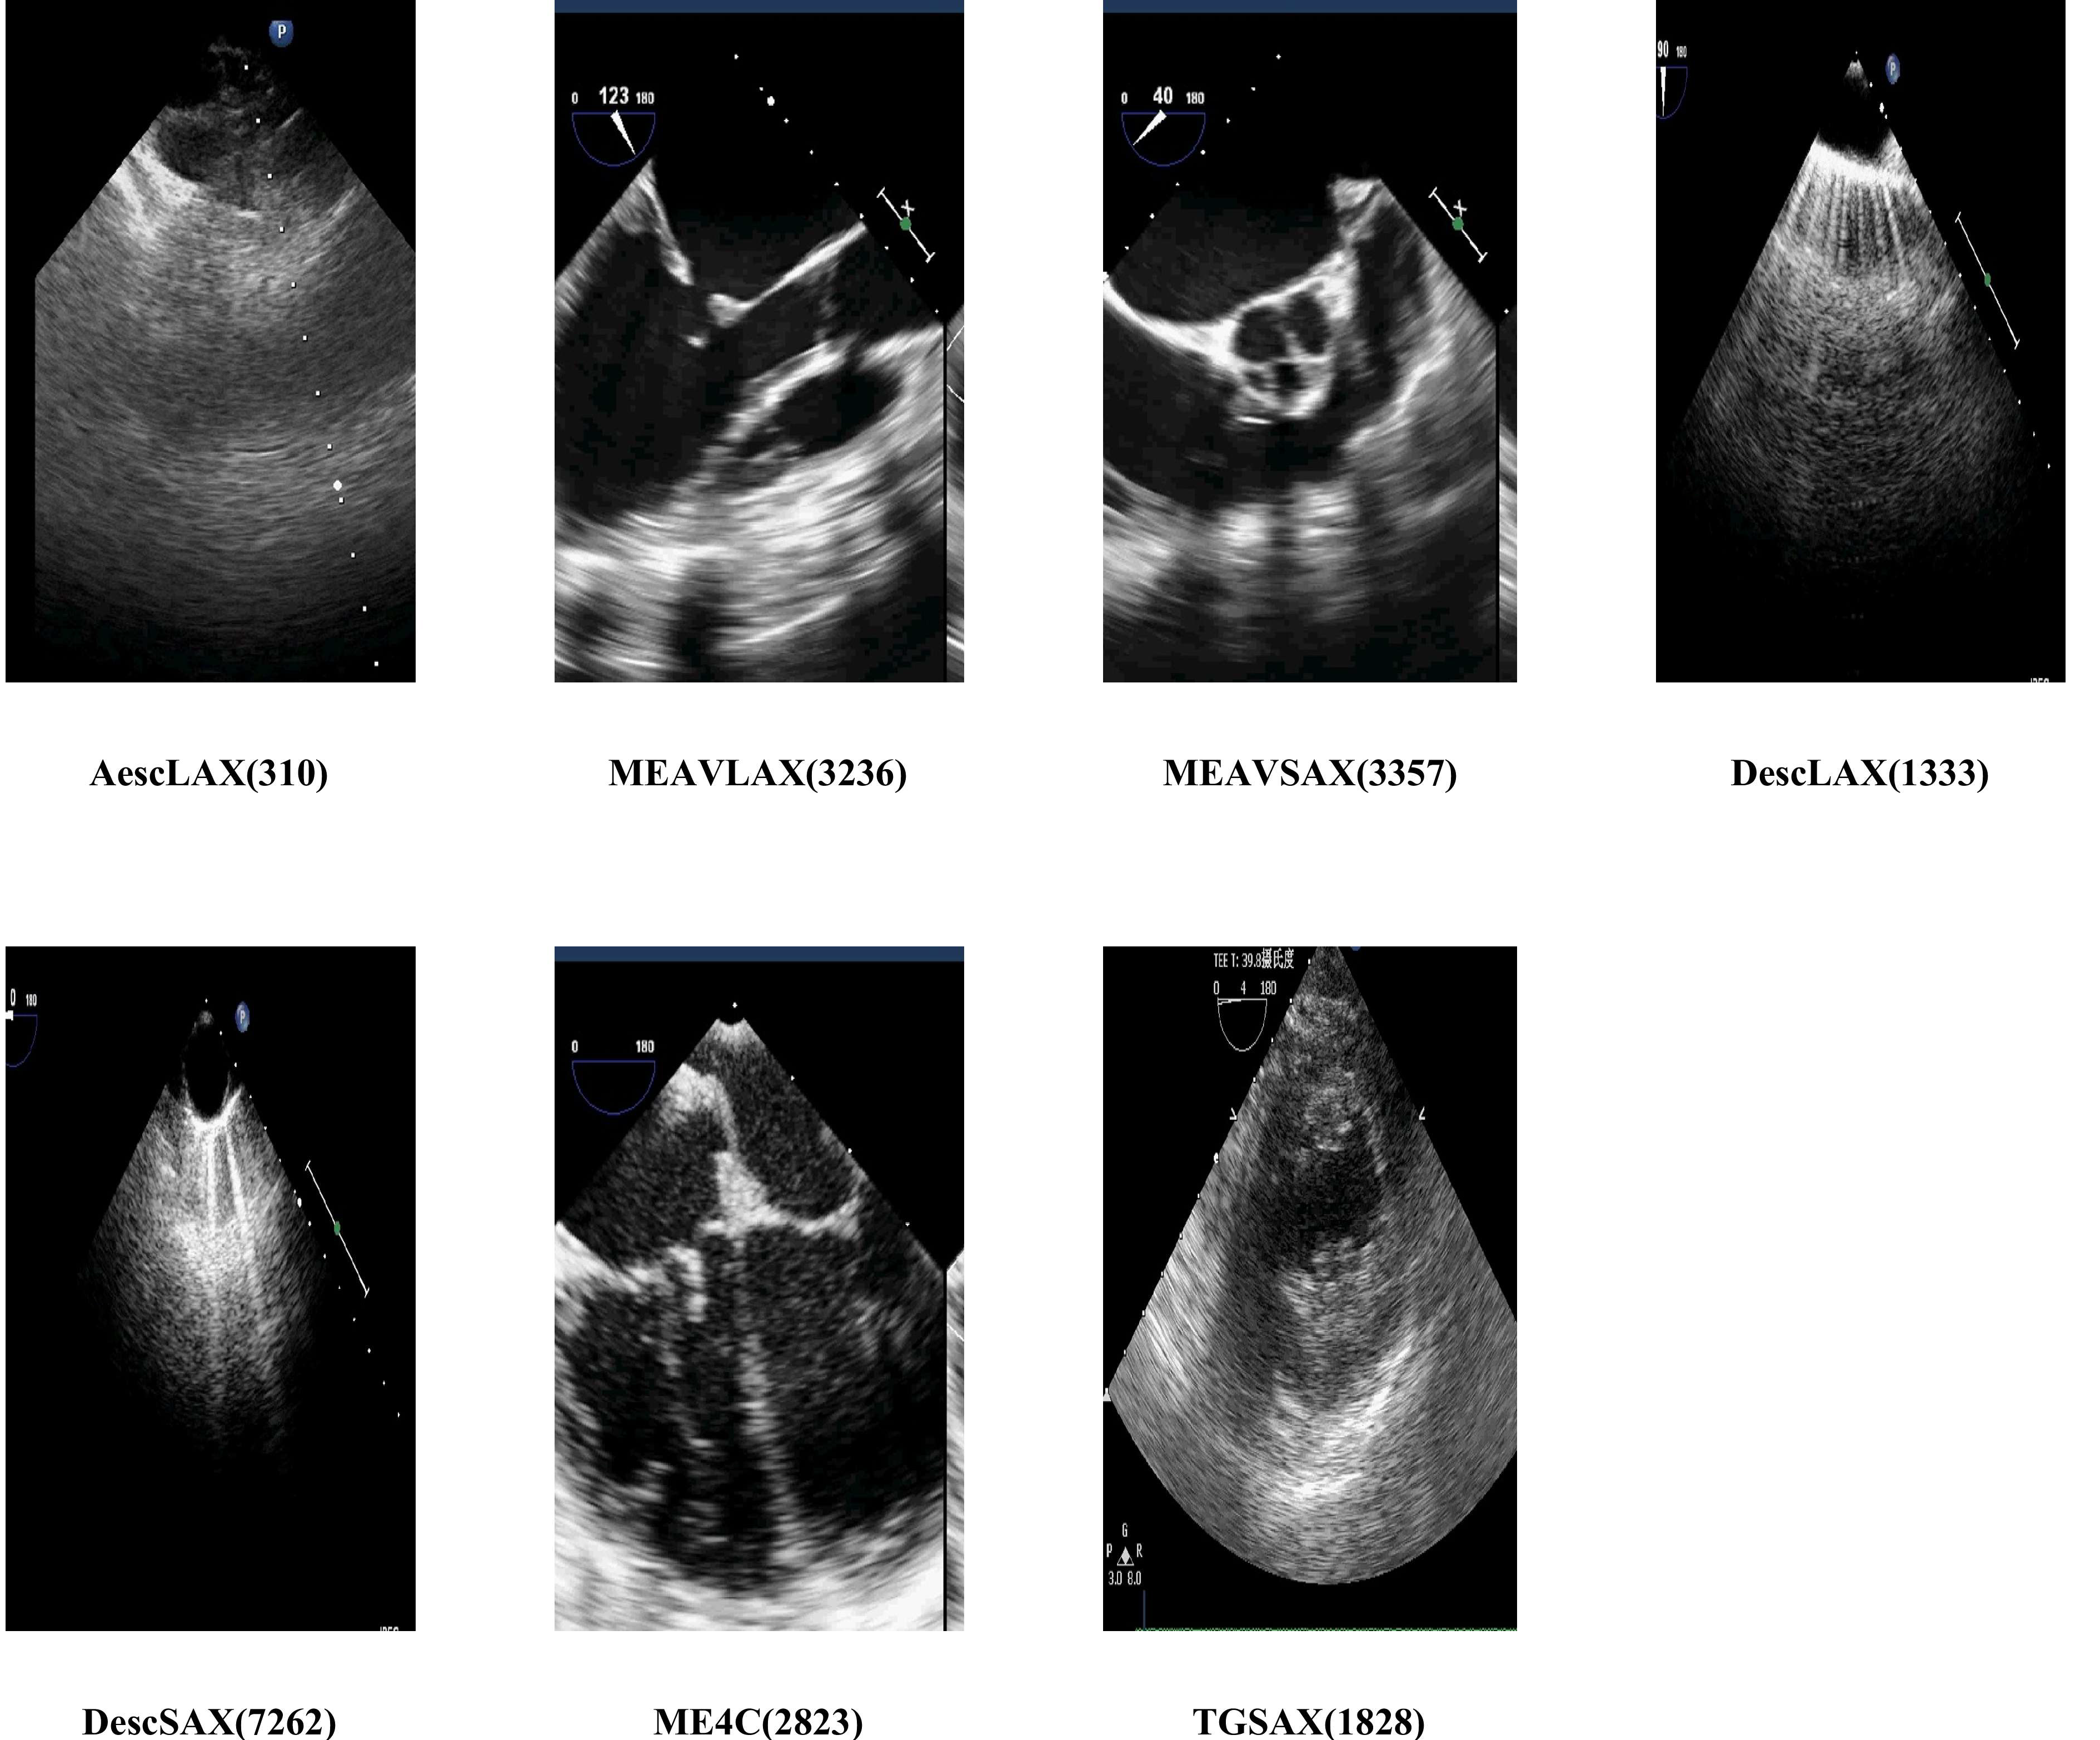
\includegraphics[trim = 30mm 0mm 30mm 0mm, clip, width=0.45\textwidth]{ch03_02}
    \includegraphics[width=0.85\textwidth]{ch02_01}
    \caption{前馈神经网络(也称为多层感知器)结构示例}
    \label{fig:ch02_01}
\end{figure}

基于极大似然估计的随机梯度下降方法是目前最常用优化的方法,它将参数$\Theta$拟合到训练集 $\mathcal{D}$。在随机梯度下降中,小批量数据的一小部分用于每个梯度更新,而不是全部数据集,在实践中优化最大可能性等价于最小化负对数似然性:
\begin{equation}
 \arg \min_{\Theta} - \sum^{N}_{n = 1} \log\big[ P(y_{n}| {\bf x}_{n}; \Theta) \big].
\end{equation}
该损失也称为分类问题的交叉熵损失,这种方法的缺点是它通常不能直接优化我们感兴趣的目标,例如ROC曲线下的面积或用于分割的常用评估度量(例如Dice系数)。

长期以来,深度神经网络(Deep Neural Network,DNN)随着层数加深导致梯度弥散问题难以有效训练。从2006年开始才重新受到欢迎\citep{Hinton2006a},两种流行的无监督网络结构:堆叠自动编码器(SAE)和深度置信网络(DBN),可以以无监督的方式逐层训练(预训练)DNN。但是,这些技术相当复杂需要大量手动调参才能产生令人满意的结果。

目前,最流行的模型是以有监督的方式进行端对端训练,通过引入预处理和新的激活函数,极大地简化了训练过程。最流行的网络结构是卷积神经网络和递归神经网络(RNN)。尽管RNN越来越受欢迎,但CNN目前在(医学)图像分析中应用最广泛。以下各节将简要介绍这些方法,从最受欢迎的方法开始,并讨论它们在应用于医疗问题时的差异和潜在的挑战。

\subsection{卷积神经网络 (CNNs)}

深度CNN是多层前馈神经网络的一种特例。隐藏层的神经元设计成跟上一层神经元局部连接,并利用参数共享来减少模型复杂度。针对图像这种结构化数据,由不同卷积核来探测不同空间位置上的局部统计特征。通过堆叠多层的卷积结构,实现从低层到高层语义空间的抽象映射。引入了感受野、卷积核滤波器组、卷积层、池化层等概念。

MLP和CNN之间有两个关键的区别:首先,网络中的权重以网络对图像执行卷积操作的方式共享。这样,模型不需要为在图像中不同位置出现的同一对象分别检测单独的检测器,从而使网络在输入的平移时保持不变性。它还大大减少了需要学习的参数数量(即权重的数量不再取决于输入图像的大小)。图\ref{fig:ch02_02}中显示了LeNet-5\citep{Jarrett2009}的经典网络结构。
\begin{figure}[!htbp]
    \centering
    %trim option's parameter order: left bottom right top
    %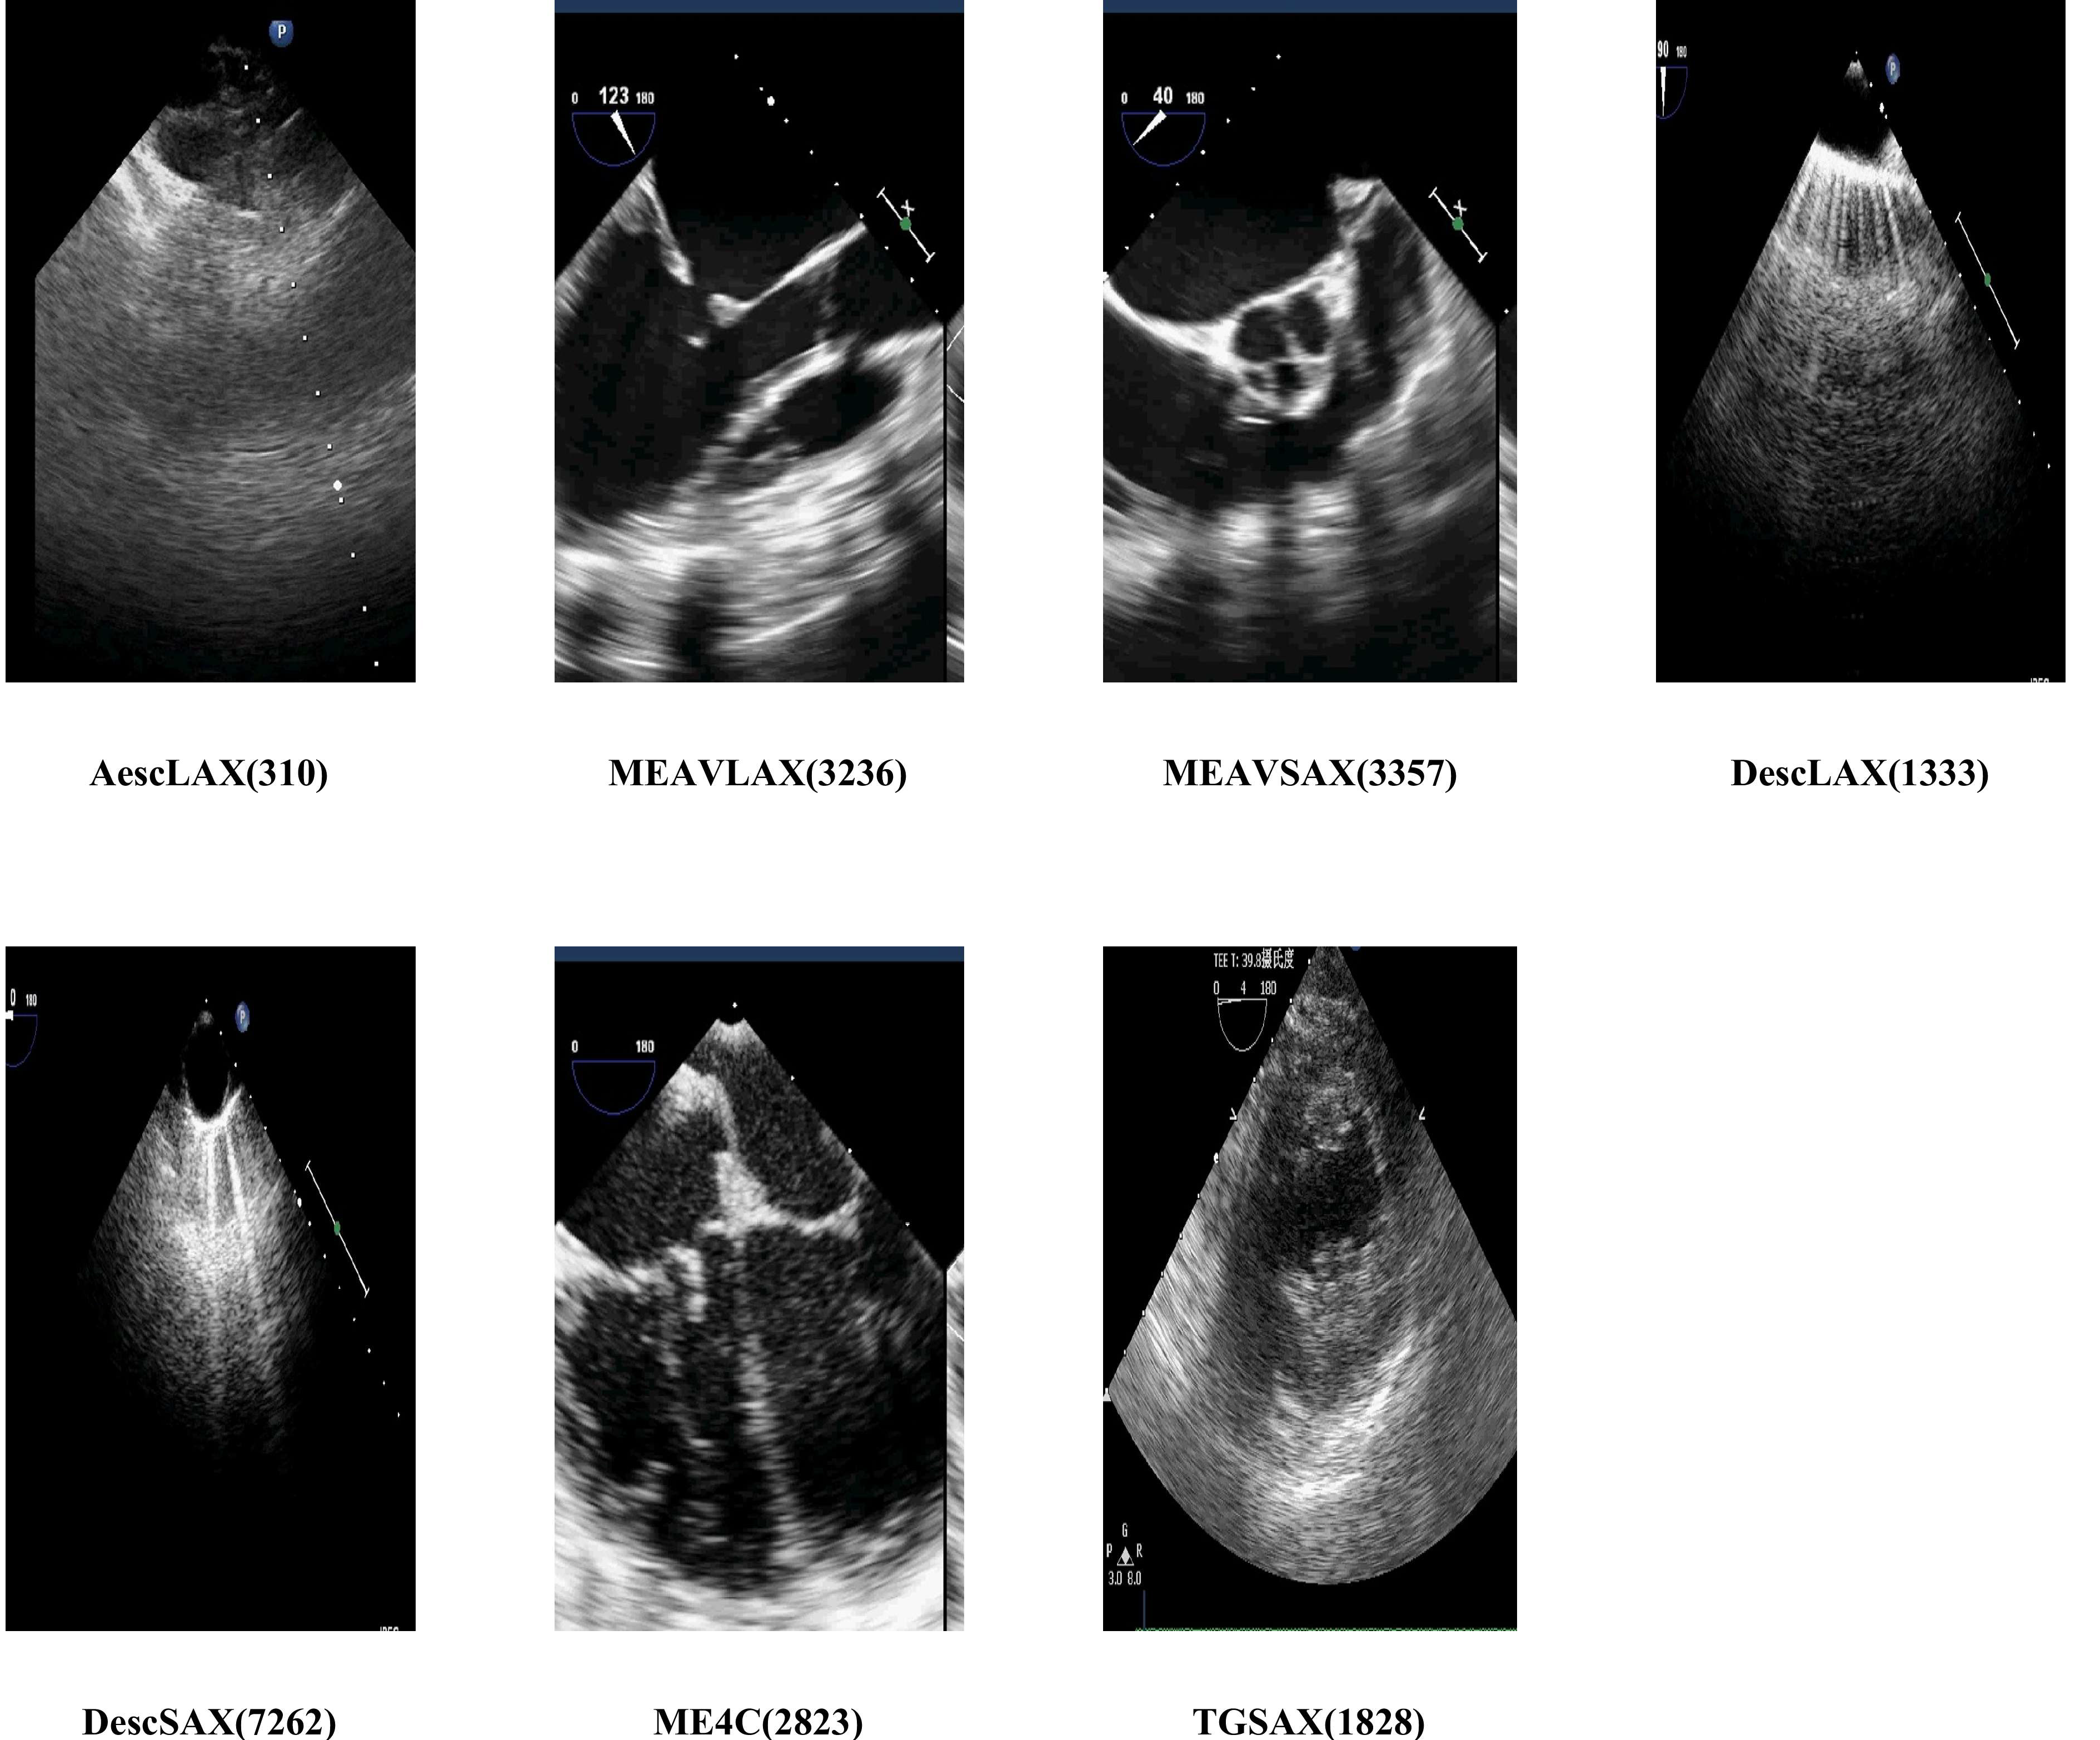
\includegraphics[trim = 30mm 0mm 30mm 0mm, clip, width=0.45\textwidth]{ch03_02}
    \includegraphics[width=0.85\textwidth]{ch02_02}
    \caption{LeNet-5网络结构示意图}
    \label{fig:ch02_02}
\end{figure}
在每一层,输入图像与一组$K$卷积核进行卷积: $\mathcal{W} = \{ {\bf W}_{1}, {\bf W}_{2}, \ldots, {\bf W}_{K} \}$ 并添加偏差项$\mathcal{B} = \{b_{1}, \ldots, b_{K}\}$,每个生成一个新的特征映射${\bf X}_{k}$。这些特征受到非线性变换$\sigma(\cdot)$的影响,并且对每个卷积层$l$重复相同的过程:
\begin{equation}
\label{eq::mapping_cnn}
 {\bf X}_{k}^{l} = \sigma\big( {\bf W}_{k}^{l -1} \ast {\bf X}^{l -1} + b_{k}^{l-1} \big).
\end{equation}

其次,在于CNN中的池化层(Pooling),其中邻域的像素值使用置换不变函数(通常是最大或平均运算)进行聚合。这会导致一定量的平移不变性,并再次减少网络中的参数数量。在网络的卷积层结束时,通常会添加全连接的层(即常规的神经网络层),其不再共享权重。类似于MLP,通过softmax函数提供最后一层中的激活值,并且使用最大可能性对网络进行训练,从而产生类别概率分布。

\subsection{深度卷积神经网络}
鉴于CNN在医学图像分析中的流行,将详细介绍广泛使用的模型中最常见的网络结构及其差异,相关的方向的演进请参考图\ref{fig:ch02_04}。
\begin{figure}[!htbp]
    \centering
    %trim option's parameter order: left bottom right top
    %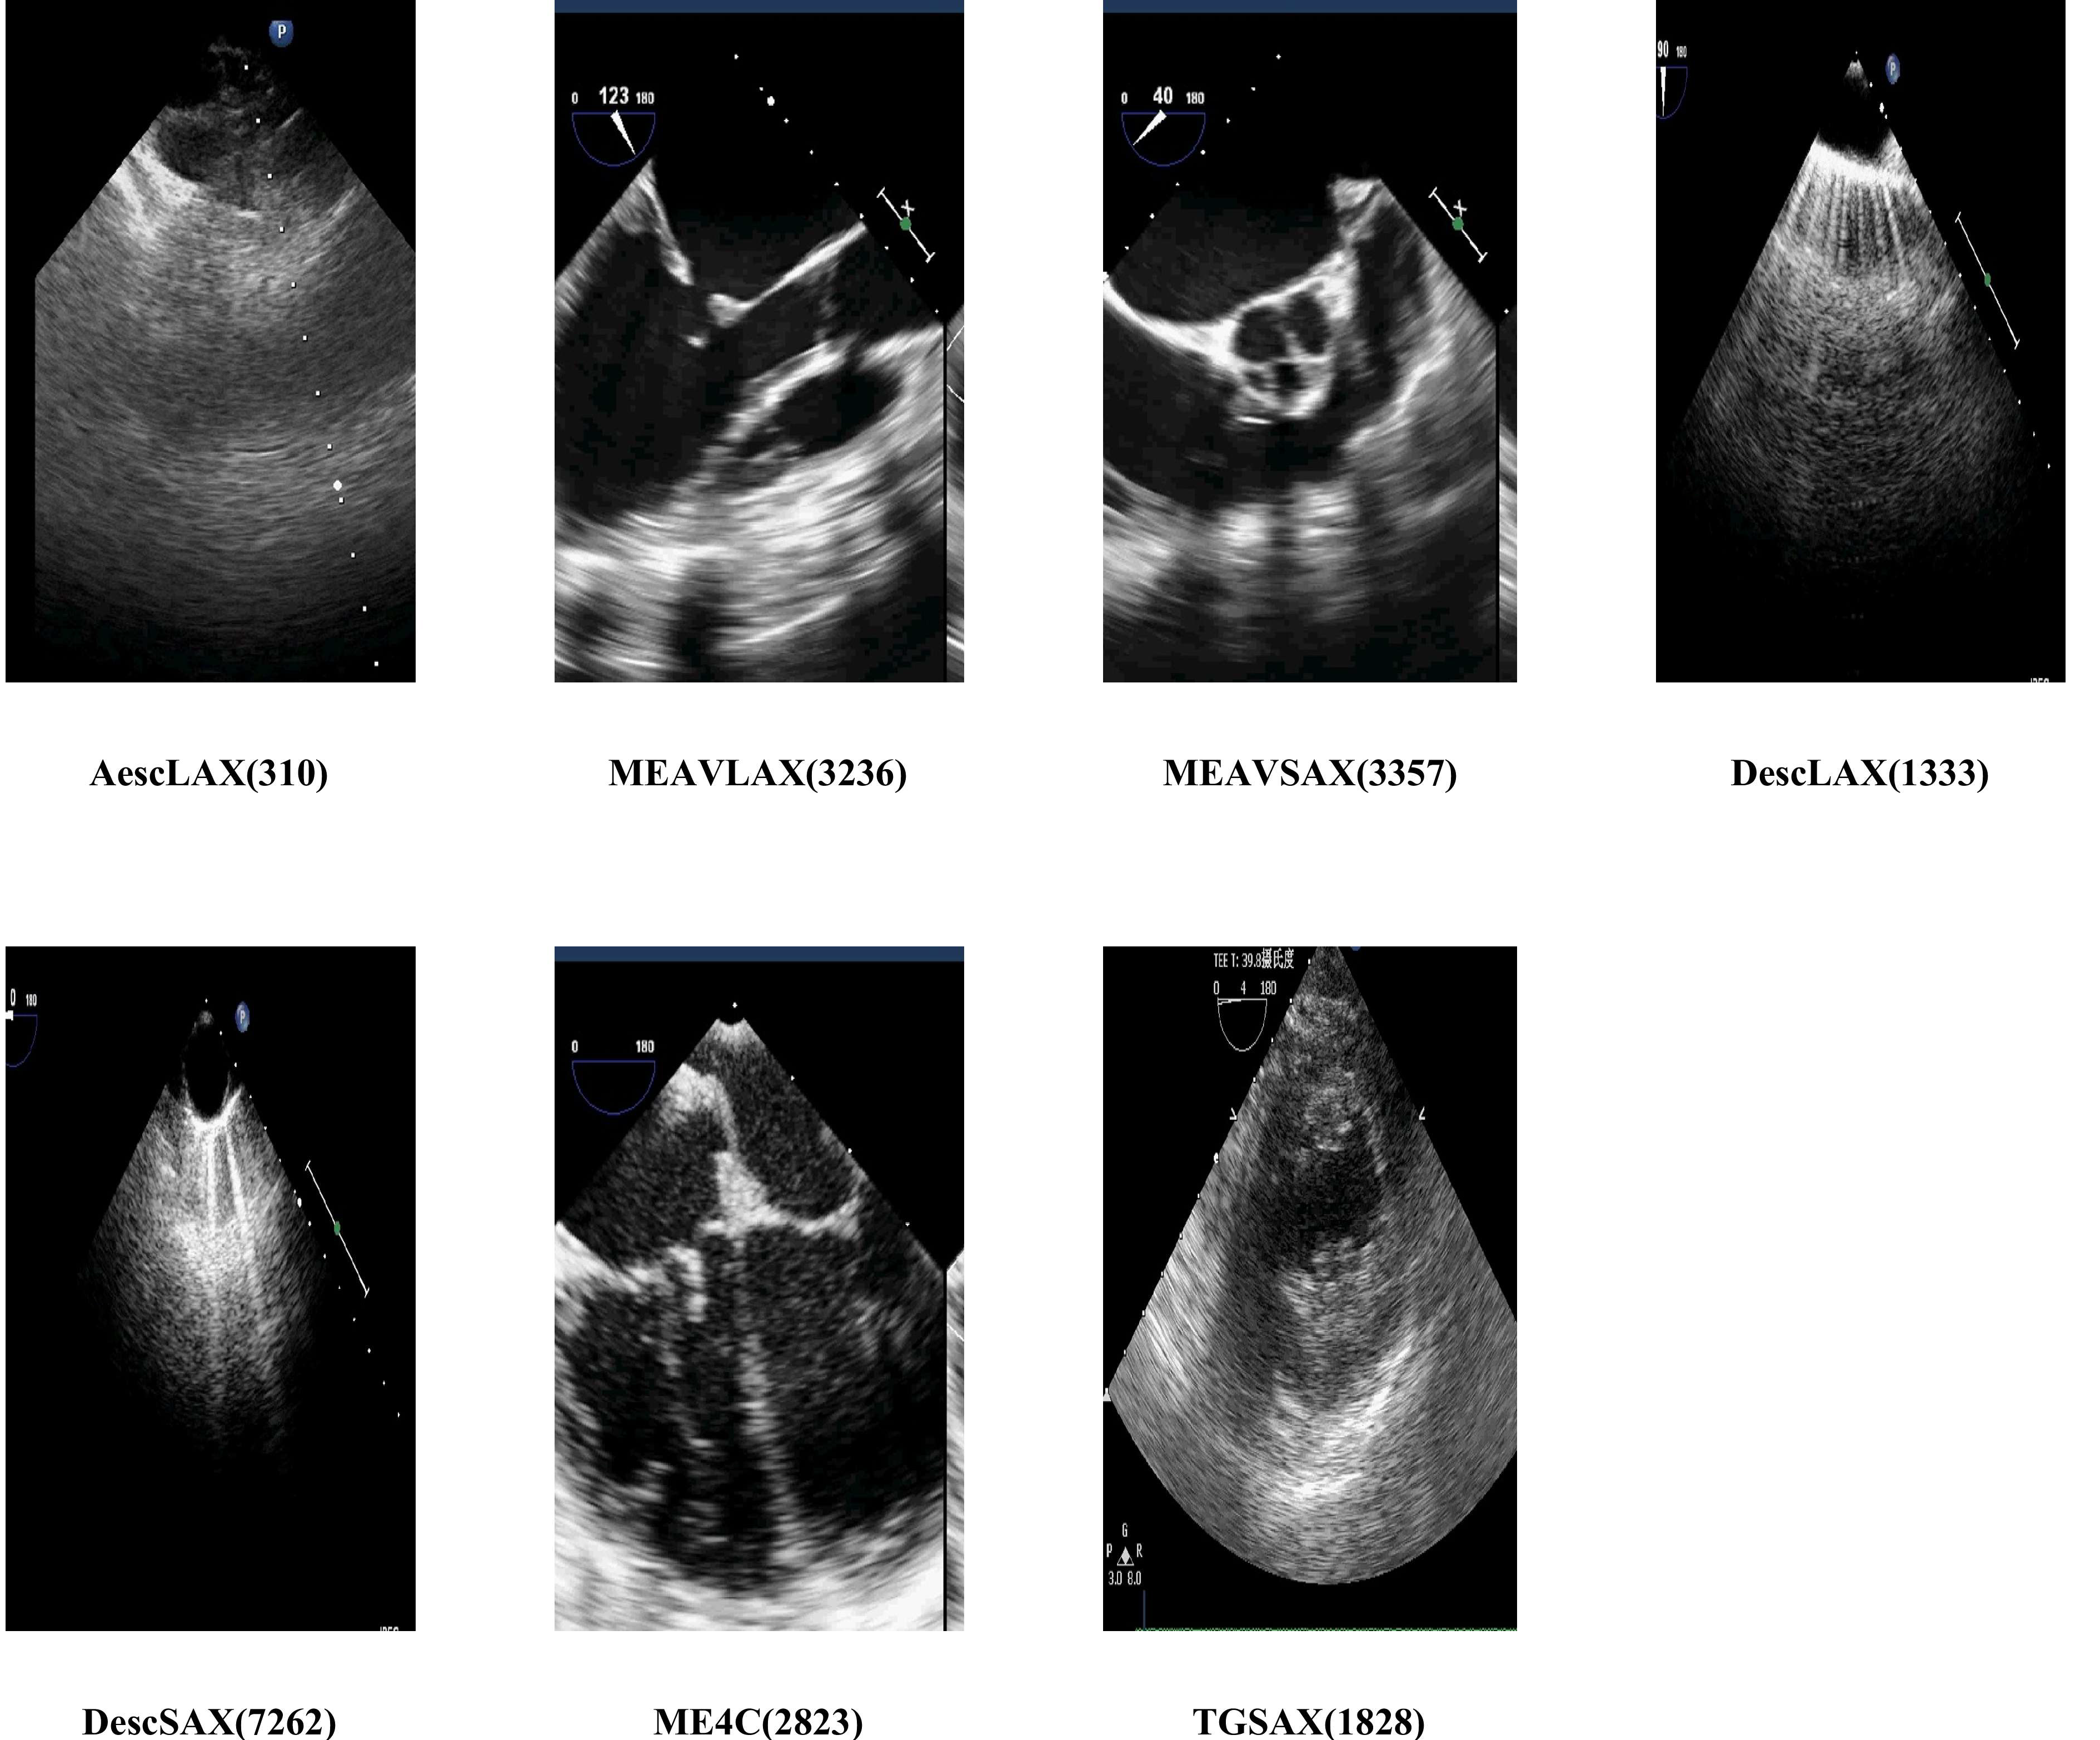
\includegraphics[trim = 30mm 0mm 30mm 0mm, clip, width=0.45\textwidth]{ch03_02}
    \includegraphics[width=0.85\textwidth]{ch02_03}
    \caption{深度卷积神经网络结构演进图}
    \label{fig:ch02_03}
\end{figure}
\subsubsection{通用分类框架}

深度CNN的典型结构AlexNet\cite{Krizhevsky2012}是在{\it LeNet}模型\citep{Jarrett2009}的基础上引入修正线性单元(Rectified Linear Units,ReLU)的激活函数和Dropout等技术\citep{Krizhevsky2012}进行了改进。模型的激活函数没有采用Sigmoid函数或双曲正切函数,而是选择ReLU函数,目的是引入更多非线性来加速训练收敛速度,解决多层网络反向传播中梯度弥散的问题。为了使得每层输入的分布更平稳,一般引入批量归一化层(Batch Normalization,BN)\cite{Ioffe2014Batch},采用最大池化层进行下采样,有时也把“卷积-激活-归一化-池化”统称为卷积层。最后需连接全连接层,全连接层就不再保存空间信息,是对低层特征的高层抽象,最终输出K维的向量,作为该图像的特征向量送入最终的分类器进行分类评估。
\begin{figure}[!htbp]
    \centering
    %trim option's parameter order: left bottom right top
    %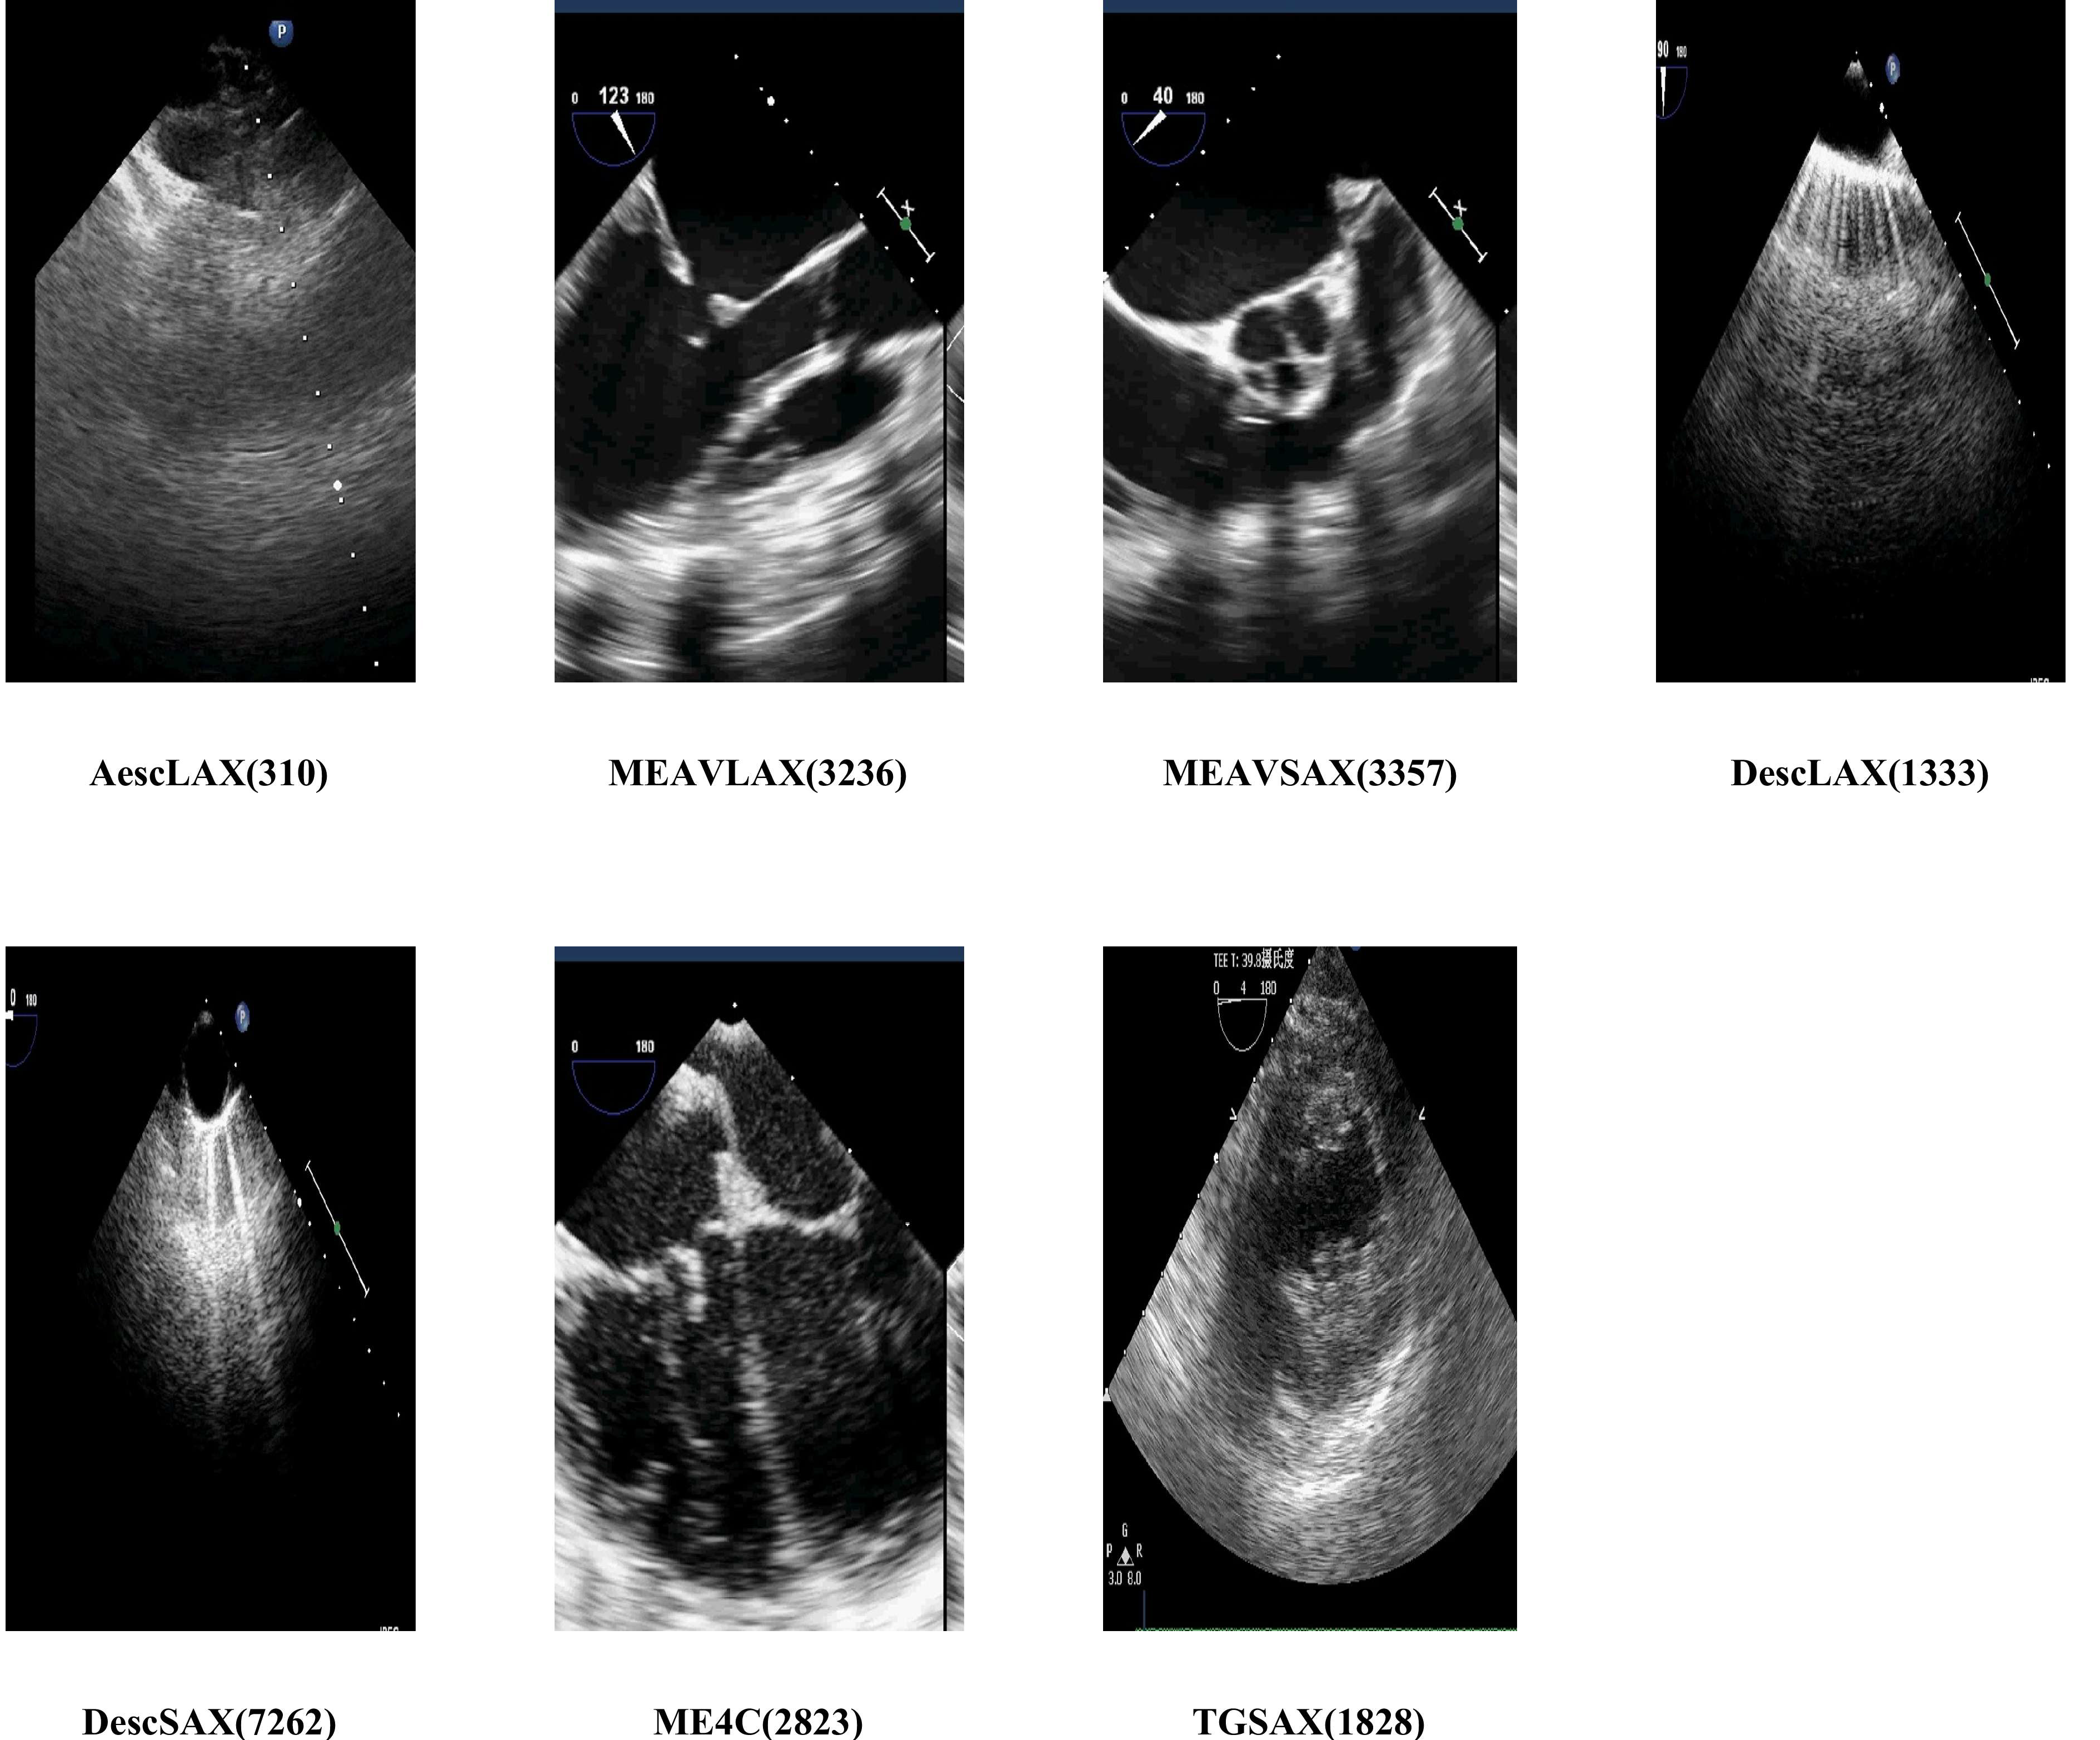
\includegraphics[trim = 30mm 0mm 30mm 0mm, clip, width=0.45\textwidth]{ch03_02}
    \includegraphics[width=0.85\textwidth]{ch02_04}
    \caption{AlexNet网络结构示意图~\cite{Krizhevsky2012}}
    \label{fig:ch02_04}
\end{figure}
 
2012年以来新的网络结构不断出现,模型更倾向于更深更复杂的结构。通过堆叠更小的卷积核,可以用较少的参数来表示类似的函数,这些更深的网络结构在推断时通常具有较低的内存占用量,这使得它们能够部署在诸如智能手机的移动计算设备上。{\it VGG}\citep{Simonyan2014a}是第一个探索更深层次的网络,并在每个层中使用$3 \times 3$的卷积核,赢得了2014年的ImageNet挑战。在深层网络之上,引入了更复杂的构建模块,可以提高训练过程的效率,并再次减少参数的数量。Szegedy等\cite{Szegedy2015}提出了一个名为{\it GoogLeNet}的22层网络,它使用使用标准密集连接结构用于估计稀疏CNN,也称为{\it Inception}模块\citep{Lin2013a},该模块使用一组不同大小的卷积$1 \times 1,3 \times 3,5 \times 5$的卷积取代了公式\eqref{eq::mapping_cnn}。类似于MLP的堆叠,这允许用较少的参数来表示类似的功能。{\it ResNet}网络结构\citep{he15}赢得了2015年的ImageNet挑战,ResNet是不同长度的网络的指数集合,其引入跳跃连接,残差块不是直接学习函数,而是仅学习残差,并因此预先调整每一层中学习接近同等函数映射,这样可以有效地训练更深的网络模型。

自2016年以来,ImageNet基准测试的性能已经饱和,很难评估性能的小幅增长是否真的归因于“更好”和更复杂的架构。这些模型所提供的较低内存占用空间的优势通常对于医疗应用来说并不重要。因此,{\it AlexNet}或其他简单模型(如{\it VGG、ResNet})仍然很受医学数据分析领域欢迎。

\subsubsection{多通路的卷积神经网络结构}
\label{sec:mc_architectures}

多个输入CNN网络的特征图可以在网络的任何处合并融合,根据不同任务需要不同融合方式可以得出多通路的网络结构。如双通道架构\cite{Kamnitsas2017}可应用于多尺度图像分析和2.5D分类。为了检测异常区域,上下文往往是一个重要的提示。增加上下文最直接的方法是将更大的区域块提供给网络,但这会显着增加网络的参数和内存需求量。因此除了提高分辨率获得局部信息之外,设计能添加上下文的网络结构:多通道多尺度网络结构首先由\cite{Farabet2013Learning}提出,将其用于自然图像分割。一些医学应用也成功地使用该概念\citep{Kamnitsas2017,Moeskops2016Automatic,Song2015Accurate,Yang2016Cascade}。

将深度学习技术应用于医疗领域的挑战通常在于将现有网络结构适应于例如不同输入格式,例如三维数据。在CNN早期应用于这样的体积数据时,通过将感兴趣体积(VOI)划分为切片,将全部3D卷积和由此产生的大量参数分开,所述切片作为不同的流馈送到网络。文献\citepns{Prasoon2013Deep}是第一个将这种方法用于膝关节软骨分割的方法。类似地,网络可以以多通道方式从3D空间中馈入多个角度的贴片\citep{Roth2014A},这些方法也被称为2.5D分类。

\subsubsection{全卷积网络结构}
\label{sec:fully_arch}

分割和去躁是自然和医学图像分析中的一项常见任务,为了解决这个问题,CNN可分别对图像中的每个像素进行分类,需要在特定像素周围提取区域块。该“滑动窗口”方法的缺点是来自相邻像素的输入块具有巨大的重叠并且多次计算相同的卷积操作,卷积和点积都是线性算子,因此内积可以写成卷积,反之亦然,通过将全连接的层重写为卷积,CNN可以输入大于其被训练的图像尺寸的任意图像,并生成概率图。但由于合并图层,这可能导致输出的分辨率远远低于输入,反卷积\citep{Long2017Fully}是为防止这种分辨率下降而提出上采样方法之一,如图\ref{fig:ch02_05}。通过将结果拼接在一起,减去由于“有效”卷积而丢失的像素,可以获得最终输出的全分辨率完整输出。
\begin{figure}[!htbp]
    \centering
    \begin{subfigure}[b]{0.45\textwidth}
        \includegraphics[height=30mm,width=\textwidth]{ch02_05_1}
        \caption{卷积}
        \label{fig:ch02_05_1}
    \end{subfigure}%
    ~% add desired spacing
    \begin{subfigure}[b]{0.45\textwidth}
        \includegraphics[height=30mm,width=\textwidth]{ch02_05_2}
        \caption{平铺卷积}
        \label{fig:ch02_05_02}
    \end{subfigure}
    ~% add desired spacing
    \begin{subfigure}[b]{0.45\textwidth}
        \includegraphics[height=30mm,width=\textwidth]{ch02_05_3}
        \caption{扩张(dilated)卷积}
        \label{fig:ch02_05_03}
    \end{subfigure}
    ~% add desired spacing
    \begin{subfigure}[b]{0.45\textwidth}
        \includegraphics[height=30mm,width=\textwidth]{ch02_05_4}
        \caption{反卷积}
        \label{fig:ch02_05_04}
    \end{subfigure}
    \caption{卷积网络中的各种卷积操作图}
    \label{fig:ch02_05}
\end{figure}
将全卷积网络进一步改进提出U-net架构\cite{Ronneberger2015},包括一个常规的全卷积结构,后面跟着一个上采样部分,其中反卷积用于增加图像大小,通过收缩编码-膨胀解码(Encoder-Decoder),将它与跳跃连接\citep{he15}相结合,以直接连接相反的Encoder-Decoder卷积层。3D数据可使用了类似的方法,\cite{Milletari2016}用于体数据的V-Net结构,提出包含类似ResNet的残余块和随机丢失(Drop)层,损失函数也不是传统的交叉熵,而是直接最小化常用的分割误差测量损失。 

\subsection{循环神经网络}
\label{sec:rnns}

传统上RNN是为处理序列数据而开发的,可以看作是MLP的泛化,输入和输出的长度都不相同,这使得它们适用于诸如机器翻译、语音识别这样的任务,其中源语言和目标语言的句子是输入和输出。在分类设置中,模型学习了给出一个可变长度序列${\bf x}_{1}, {\bf x}_{2}, \ldots, {\bf x}_{T}$的类别$P(y | {\bf x}_{1}, {\bf x}_{2}, \ldots, {\bf x}_{T}; \Theta)$,而不是一个输入向量${\bf x}$。

普通的RNN在$t$时刻维持一个隐式或隐藏状态${\bf h} $,它是从其输入${\bf x}_{t}$和前一状态${\bf h}_{t-1}$:
\begin{equation}
 {\bf h}_{t} = \sigma({\bf W}{\bf x}_{t} + {\bf R}{\bf h}_{t - 1} + {\bf b}),
\end{equation}

其中加权矩阵${\bf W}$和${\bf R}$是随时间共享的。对于分类,通常会添加一个或多个完全连接的层,然后添加softmax以将序列映射到类别概率: 
\begin{equation}
 P(y | {\bf x}_{1}, {\bf x}_{2}, \ldots, {\bf x}_{T}; \Theta) = \text{softmax}( {\bf h}_{T}; {\bf W}_{out}, {\bf b}_{out}).
\end{equation}

由于梯度需要通过时间从输出反向传播,因此RNN具有固有的深度(及时性),因此与常规深层神经网络一样遭受梯度弥散难以训练问题。为此已经设计几种专用单元来解决上下文依赖问题,最早和最流行的是长期短期记忆(Long Short-Term Memory,LSTM)单元\citep{Hochreiter1997Long},而门控复发单元(Gated Recurrent Unit,GRU)\citep{Cho2014Learning}是LSTM的最新简化版。

尽管最初提出是针对一维输入,但RNN越来越多地应用于图像,在自然图像中,“pixelRNN”被用作自回归模型,生成模型最终可以生成类似于训练集样本的新图像。对于医疗应用,它们已被用于分割问题,并且在各种竞赛挑战中具有令人鼓舞的结果\citep{Stollenga2015Parallel}。

\subsection{无监督深度学习}
\subsubsection{自编码器}
自编码器(Auto-encoders,AE)是简单神经网络的一种,通过一个隐藏层${\bf h}$来产生编码(code)${\bf x}'$近似表示输入${\bf x}$。重建其隐藏层${\bf W}_{h, x'}$ 和相应的偏差$b_{h, x'}$,它们由权重矩阵和输入到隐藏状态和${\bf W}_{x, h}$的偏置$b_{x, h}$来控制。非线性函数用于计算隐藏激活: 
\begin{equation}
\label{eq::ae_projection}
 {\bf h} = \sigma({\bf W}_{x, h} {\bf x} + {\bf b}_{x, h}).
\end{equation}
此外,隐藏层$|{\bf h}|$的维度小于$|{\bf x}|$。这样,数据被投影到表示输入中的主要潜在结构的较低维子空间上。如果隐藏层的大小与输入大小相同,并且不再添加非线性,则模型将简单地学习标识函数,正则化或稀疏性约束可以用来增强发现过程。

去噪自动编码器\citep{Vincent2010Stacked}是另一种防止模型学习微不足道解决方案的解决方案。这里模型被训练来重构来自噪声损坏版本(通常是盐和胡椒噪声)的输入。SAE(或深度AE)通过将自动编码器层放置在彼此之上而形成。相关医疗应用中,自动编码器层经常被(“贪婪算法”)单独训练,然后使用监督训练对整个网络进行微调以进行预测。

\subsubsection{受限波兹曼机和深度信念网络}
受限玻尔兹曼机(Restricted Boltzmann Machines,RBMs)\citep{Hinton2006a}是一种马尔可夫随机场,构成输入层或可见层${\bf x} = (x_{1}, x_{2}, \ldots, x_{N})$和一个带有潜在特征表示的隐藏层${\bf h} = (h_{1}, h_{2}, \ldots, h_{M})$。节点之间的连接是双向的,因此给定输入向量$\bf x$可以获得潜在特征表示$\bf h$,反之亦然。因此,RBM是一个生成模型,我们可以从中进行抽样并生成新的数据点。与物理系统类比,能量函数被定义为输入和隐藏单位的特定状态$({\bf x}, {\bf h})$:
\begin{equation}
 E({\bf x}, {\bf h}) = {\bf h}^{T}{\bf W}{\bf x} - {\bf c}^{T}{\bf x} - {\bf b}^{T}{\bf h},
\end{equation}
与 ${\bf c}$ and ${\bf b}$ 偏差条款。系统的“状态”的概率通过将能量传递给指数和正态化来定义:
\begin{equation}
 p({\bf x}, {\bf h}) = \frac{1}{Z} \exp\{ - E({\bf x}, {\bf h}) \}.
\end{equation}
计算分区函数 $Z$通常是棘手的。然而,以${\bf h}$为条件计算${\bf v}$形式的条件推断是可以处理的,并且会产生一个简单的公式:
\begin{equation}
 P(h_{j} | {\bf x}) = \frac{1}{ 1 + \exp\{ -b_{j} - {\bf W}_{j}{\bf x}\} }.
\end{equation}
由于网络是对称的,类似的表达式适用 $P(x_{i} | {\bf h})$.

DBNs \citep{Hinton2009Deep}实质上是AE层被RBM取代的堆叠多层AE。再次,以无人监督的方式进行单个层次的训练。通过向DBN顶层添加线性分类器并执行监督优化来执行最终的微调。
\subsubsection{变分自编码器和深度生成对抗网络}
最近,引入了两种新颖的无监督网络结构:变分自动编码器(VAE)\citep{Kingma2013Auto}和生成对抗网络(GAN)\citep{Goodfellow2014Generative}。因很难解决它们配分函数的数值而成为众所周知的难题,目前还没发现将这些方法应用于医学图像,但在自然图像中的应用还是值得期待的。

\section{深度学习核心技巧}
\subsection{激活函数和优化方法}

\subsection{正则化}

\section{相关软硬件平台}
GPU和GPU计算库(CUDA,OpenCL)的广泛应用促成了深度学习急剧上升的主要原因之一。GPU是高度并行计算引擎,其执行线程数量比中央处理器(CPU)多一个数量级。使用目前的硬件,深度学习GPU的速度通常比CPU快10到30倍。FPGA和定制的深度学习芯片也获得了相当的关注。

除硬件之外,深度学习方法普及的另一推动力是开源软件库和共享深度模型的广泛可用性。这些库提供了神经网络中重要操作(如卷积、循环网络)的高效GPU实现方便用户使用。当前流行的软件包是(按字母顺序):
\begin{itemize}
 \item {\bf Caffe} \citep{Jia2014}. 提供C ++和Python接口,由加州大学伯克利分校的研究生开发。
 \item {\bf Tensorflow} \citep{Abadi2016TensorFlow}. 由Google开发提供C ++,Python和接口.
 \item {\bf Theano} \citep{AlRfou2016Theano}. 提供由蒙特利尔MILA实验室开发的Python库。
 \item {\bf Mxnet} \citep{Chen2015mxnet}. 提供一个Lua接口,并被其他人用于Facebook AI研究 
\end{itemize}
 
\section{小结与讨论}

 